% !TeX program = xelatex
\documentclass[runningheads]{llncs}
\usepackage[paperheight=295mm,paperwidth=210mm]{geometry}
\usepackage{graphicx}
\usepackage{wrapfig}
\usepackage{import}
\usepackage{kotex}
\usepackage[dvipsnames]{xcolor}
\usepackage{fancyvrb} %
\usepackage{listings}
\usepackage{tabularx}
\usepackage{underscore}
\usepackage{multicol}
\usepackage{enumitem}
\usepackage{subcaption}
\usepackage[numbers,square,super]{natbib}
\usepackage{mathptmx} % Times New Roman
\usepackage{amsmath}
\usepackage{amssymb}
\usepackage{framed}
\usepackage{etoolbox}
\usepackage{cancel}
\usepackage{physics}
\usepackage{tikz}
\usepackage{parskip}
\usepackage{enumerate}
\usepackage{minted}
\usepackage{inconsolata}
\usepackage{makecell}
\usepackage{slashed}
\usepackage{nicematrix}
\usetikzlibrary{calc, angles, quotes, graphs, positioning, arrows}

\setcounter{tocdepth}{2}

\colorlet{shadecolor}{gray!30}

\newcommand\enclosebox[2]{%
  \BeforeBeginEnvironment{#1}{\begin{#2}}%
  \AfterEndEnvironment{#1}{\end{#2}}%
}

\enclosebox{theorem}{oframed}
\enclosebox{definition}{leftbar}

\newcommand{\divides}{\bigm|}
\newcommand{\ndivides}{%
  \mathrel{\mkern.5mu % small adjustment
    % superimpose \nmid to \big|
    \ooalign{\hidewidth$\big|$\hidewidth\cr$\nmid$\cr}%
  }%
}
\newcommand{\ord}{\operatorname{\mathrm{ord}}}
\newcommand{\ind}{\operatorname{\mathrm{ind}}}
\newcommand{\legendre}[2]{\left(\frac{#1}{#2}\right)}
\setmainfont{Times New Roman}
\setmainhangulfont{Nanum Myeongjo}
\setmonofont{SF Mono}
\setlength{\parindent}{1em}
\setlength{\parskip}{0pt}
\linespread{1.2}
%\renewcommand{\arraystretch}{1.5}
\setlength{\tabcolsep}{0.5em}%
\newenvironment{Figure}
  {\par\medskip\noindent\minipage{\linewidth}}
  {\endminipage\par\medskip}
\newcommand{\translation}[1]{\textsuperscript{#1}}

\makeatletter
\renewcommand\NAT@citesuper[3]{\ifNAT@swa
\if*#2*\else#2\NAT@spacechar\fi
\unskip\kern\p@\textsuperscript{\NAT@@open#1\if*#3*\else,\NAT@spacechar#3\fi\NAT@@close}%
   \else #1\fi\endgroup}
\makeatother

\let\oldtabular\tabular% Store a copy of \tabular
\let\endoldtabular\endtabular% Store a copy of \endtabular
\renewenvironment{tabular}[2][\arraystretch]
  {\edef\arraystretch{#1}% Update \arraystretch
   \oldtabular{#2}}% \begin{tabular}[<stretch>]{<col spec>}
  {\endoldtabular}% \end{tabular}

\begin{document}

\title{Discrete Mathematics (0034)\newline\space Lecture Notes}
\author{Yulwon Rhee (202211342)}
\institute{Department of Computer Science and Engineering, Konkuk University}

\maketitle
\section{Week 1}
\subsection{논리와 명제}
논리 : 사고의 규칙\\
명제 논리(Propositional Logic): T/F 판별 가능한 문장 or 수식\\
술어 논리(Predicate Logic): 변수 포함 명제\\
단순 명제(Simple Proposition): 하나의 문장 or 수식으로 구성된 명제\\
합성 명제(Composition Proposition): 단순 명제들이 논리 연산자로 연결\\\\
항진 명제(Tautology): 항상 T인 합성 명제\\
모순 명제(Contradiction): 항상 F인 합성 명제\\
\subsection{논리 연산자}
\begin{table}[]
    \begin{minipage}{\linewidth}
        \caption {Logical Operators}
        \centering
        \begin{tabular}[1.5]{c|c}
        연산자      & 기호\\
        \Xhline{3\arrayrulewidth}
        부정(NOT)  & $\sim$\\
        \hline
        논리곱(AND) & $\land$\\
        \hline
        논리합(OR)  & $\lor$\\
        \hline
        배타적 논리합(XOR)&$\oplus$\\
        \hline
        조건(if then)&$\to$\\
        \hline
        쌍방 조건(iff)&$\leftrightarrow$
        \end{tabular}
    \end{minipage}
\end{table}
\begin{table}[]
    \caption {Truth Table for the XOR, Implication and Biconditional Proposition}
    \begin{minipage}{.33\linewidth}
        \centering
        \begin{tabular}[1.5]{cc|c}
        $p$&$q$&$p\oplus q$\\
        \Xhline{3\arrayrulewidth}
        T&T&F\\
        T&F&T\\
        F&T&T\\
        F&F&F
        \end{tabular}
    \end{minipage}
    \begin{minipage}{.33\linewidth}
        \centering
        \begin{tabular}[1.5]{cc|c}
        $p$&$q$&$p\to q$\\
        \Xhline{3\arrayrulewidth}
        T&T&T\\
        T&F&F\\
        F&T&T\\
        F&F&T
        \end{tabular}
    \end{minipage}
    \begin{minipage}{.33\linewidth}
        \centering
        \begin{tabular}[1.5]{cc|c}
        $p$&$q$&$p\leftrightarrow q$\\
        \Xhline{3\arrayrulewidth}
        T&T&T\\
        T&F&F\\
        F&T&F\\
        F&F&T
        \end{tabular}
    \end{minipage}
\end{table}
\newpage
\begin{itemize}
    \item $p$이면 $q$이다. (if $p$ then $q$, $q$ when $p$, $p$ only if $q$)
    \item $p$는 $q$의 충분조건이다. ($p$ is sufficient for $q$)
    \item $q$는 $p$의 필요조건이다. ($q$ is necessary for $p$)
    \item $p$는 $q$를 함축한다. ($p$ implies $q$)
\end{itemize}

\subsection{논리 연산자 우선순위}
$$\sim\quad>\quad\land\quad>\quad\lor\quad>\quad\to\quad>\quad\leftrightarrow$$
\subsection{논리 연산: 상호 관계}
\begin{table}[]
    \caption {$p\to q$에 대하여}
    \centering
    \begin{tabular}[1.5]{c|c}
        역(Converse)&$q\to p$\\
        \hline
        이(Inverse)&$\sim p \to \sim q$\\
        \hline
        대우(Contrapositive)&$\sim q \to \sim p$
    \end{tabular}
\end{table}
\subsection{예제 풀이}
e.g.) You cannot ride the rollercoaster if you are under 4 ft. tall unless you are older than 16 years old.\\
$p$ : You can ride the rollercoaster\\
$q$ : You are under 4 ft. tall\\
$r$ : You are older than 16 years old\\
$\sim p$ if $q$ unless $r$\\$\Rightarrow$ $\sim p$ if $q$ if $\sim r$\\$\Rightarrow$ $\sim r \to (q \to \sim p)\\\equiv (\sim r \land q) \to \sim p$\\
\newpage
\section{Week 2}
\subsection{비트 연산(Bit Operations)}
\begin{table}[]
    \caption {Logical Operators}
    \centering
    \begin{tabular}[1.5]{c|c|c|c|c|c|c}
    Name      & NOT & AND & OR & XOR & Implies & Iff\\
    \Xhline{3\arrayrulewidth}
    Propositional Logic & $\sim$ & $\land$ & $\lor$ & $\oplus$ & $\to$ & $\leftrightarrow$\\
    \hline
    Boolean Algebra & $\overline{p}$ & $p\cdot q$ & $+$ & $\oplus$ & &\\
    \hline
    C/C++/Java(Wordwise) & \texttt{!} & \texttt{\&\&} & \texttt{||} & \texttt{!=} & & \texttt{==}\\
    \hline
    C/C++/Java(Bitwise) & \texttt{ \~} & \texttt{\&} & \texttt{|} & \texttt{ \^} & &\\
    \end{tabular}
\end{table}
\subsection{논리적 동치 관계}
$p\leftrightarrow q$가 항진 명제 $\to$ $p, q$는 논리적 동치, $p \equiv q$ 또는 $p \Leftrightarrow q$\\
\begin{table}[]
    \caption {논리적 동치 관계}
    \centering
    \begin{tabular}[1.5]{c|c}
        법칙 이름&동치 관계\\
        \Xhline{3\arrayrulewidth}
        결합 법칙&\begin{tabular}[1.5]{@{}c@{}}$(p\lor q)\lor r \equiv p \lor (q \lor r)$\\$(p\land q)\land r \equiv p \land (q \land r)$\end{tabular}\\
        \hline
        홀수 법칙&\begin{tabular}[1.5]{@{}c@{}}$p\lor(p\land q) \equiv p$\\$p\land(p\lor q) \equiv p$\end{tabular}\\
        \hline
        드 모르간 법칙&\begin{tabular}[1.5]{@{}c@{}}$\sim(p\lor q)\equiv(\sim p)\land(\sim q)$\\$\sim(p\land q)\equiv(\sim p)\lor(\sim q)$\end{tabular}\\
        \hline
        조건 법칙& $p\to q\equiv\sim p\lor q$\\
        \hline
        대우 법칙& $p\to q\equiv\sim q\to\sim p$
    \end{tabular}
\end{table}
\newpage
\subsection{술어 논리(Predicate Logic)}
$p(x)=x$에 대한 명제술어
\subsection{술어 한정자(Predicate Quantifier)}
$\forall$: 모든\\
$\exists$: 어떤\\
괄호를 이용하여 모순이 없도록 범위 지정 필요\\
제한된 정의역 표현: 변수가 만족해야 하는 조건이 한정기호 다음에 표기\\
e.g.) $$\forall x<0(x^2>0)\text{, 정의역은 실수 }\Longrightarrow \forall x (x < 0 \rightarrow x^2>0)$$
$$\exists x>0(x^2=2)\text{, 정의역은 실수 }\Longrightarrow \exists x(x>0 \land x^2=2)$$
\\
부정:
$$\sim \forall(p(x)) \equiv \exists x(\sim p(x))$$
$$\sim (\exists x p(x)) \equiv \forall x(\sim p(x))$$

\subsection{중첩 한정자}
$\forall x \exists y\ P(x, y)$: For every $x$, there is a $y$ for which $P(x, y)$ is true.\\
$\exists x \forall y\ P(x, y)$: There is an $x$ for which $P(x, y)$ is true for every $y$.

\subsection{예제 풀이}
1. If a user is active at least one network link will be available.

$A(u)$ : User $u$ is active.

$S(n, x)$ : Network link $n$ is in status $x$.

$\exists u\ A(u) \to \exists n\ S(n, \text{available})$\\\\
2. Everyone has exactly one best friend.
\begin{itemize}[label=$\to$]
    \item For every person $x$, person $x$ has exactly one best friend.
    \item 'Exactly one' means that
    \begin{itemize}
        \item[1.] There is a person $y$ who is the best friend of $x$.
        \item[2.] For every person $z$, if person $z$ is not $y$, then $z$ is not the best friend of $x$.
    \end{itemize}
\end{itemize}

$B(x, y)$: $y$ is the best friend of $x$.

$\forall x \exists y (B(x, y))$, $y$의 조건: $\forall z((z\neq y) \to \sim B(x, z))$\\\\
$L(x, y)$: $x$ loves $y$.\\
3. There is somebody whom everybody loves.

$\exists y\forall x\ L(x, y)$ ($\exists y$와 $\forall x$ 순서 유의!)\\
4. Nobody loves everybody

$\sim \exists x \forall y\ L(x, y) \equiv \forall x \exists y\ \sim L(x, y)$
\section{Week 3}
\subsection{추론}
(연역적) 추론(Argument): 주어진 명제 $p_n$을 바탕으로 새로운 명제 $q$를 유도

$p_n$: 전제(Premise), 가정(Hypothesis)

$q$: 결론(Conclusion)\\
유효 추론(Valid Argument): 전제 T, 결론 T\\
허위 추론(Fallacious Argument): 결론 F
\begin{table}[H]
    \caption {논리적 추론 법칙}
    \centering
    \begin{tabular}[1.5]{c|c}
        법칙 이름&추론 법칙\\
        \Xhline{3\arrayrulewidth}
        긍정 법칙*&$p,\ p\to q\vdash q$\\
        \hline
        부정 법칙*&$\sim q,\ p \to q\vdash \sim p$\\
        \hline
        조건 삼단 법칙*&$p \to q,\ q \to r\vdash p \to r$\\
        \hline
        선언 삼단 법칙&$p \lor q,\ \sim p\vdash q$\\
        \hline
        양도 법칙&$(p\to q)\land(r\to s),\ p\lor r\vdash (q\lor s)$\\
        \hline
        파괴적 법칙&$(p\to q)\land(r\to s),\ \sim q \lor \sim s\vdash \sim p \lor \sim r$\\
        \hline
        선접 법칙&$p \vdash p \lor q$\\
        \hline
        분리 법칙&$p \land q\vdash p$\\
        \hline
        연접 법칙&$p,\ q\vdash p \land q$
    \end{tabular}
    \\
    \bigskip
    * 가장 많이 사용되고 잘 알려진 3가지 법칙
\end{table}
\subsection{대치 vs 추론}
대치의 공식은 합성 명제 전체 또는 한 부분에 적용 가능\\
추론의 법칙은 합성 명제의 주 연산자에 사용

\subsection{증명법: 한정기호를 사용한 명제의 추론규칙}
전칭 예시화(Universal Instantiation): $\forall x P(x) \to \exists c P(c)$\\
전칭 일반화(Universal Generalisation): $P(c)\text{ for an arbitrary }c \to \forall x P(x)$\\
존재 예시화(Existential Instantiation): $\exists x P(x) \to P(c)$ for some $c$ ($c$가 적어도 하나 존재)\\
존재 일반화(Existential Generalisation): $P(c)$ for some $c \to \exists x P(x)$

\subsection{정리의 증명}
정의: 논의 대상 보편화 위해 사용 용어 or 기호 의미를 확실히 규명한 문장 or 식

e.g.) 한 내각의 크기가 직각인 삼각형은 직각삼각형, 명제는 T/F 판별 가능한 문장 or 수식\\
공리: 별도 증명 없이 T로 이용되는 명제

e.g) $p$가 참이면 $p\lor q$도 참, $a=b$면, $a+c=b+c$\\
정리: 공리, 정의로 T가 확인된 명제\\
증명: 공리, 정의, 정리로 명제가 T임을 확인하는 과정

\subsection{증명 방법}
$p\to q$ 증명: $p, q$ 모두 T or $p$ 무조건 거짓\\
직접 증명법: $p\to q$ 직접 증명\\
간접 증명법: 동치로 $p \to q$ 변환하여 증명. 대우 증명법, 모순 증명법, 반례 증명법, 존재 증명법\\
기타 증명법: 수학적 귀납법

\subsection{수학적 귀납법}
연역법(Deduction): 사실(Fact), 공리(Axiom)에 입각해 추론(Inference)을 통해 새로운 사실 도출\\
귀납법(Induction): 관찰, 실험에 기반한 가설을 귀납 추론을 통해 일반적인 규칙으로 입증

\subsection{예제 풀이}
1. There is someone in this class who has been to France

Everyone who goes to France visits the Louvre.

Therefore, someone in this class has visited the Louvre.
\subsubsection{Solution.}\hphantom{}

$x$: 사람

$C(x): x$ is in this class.

$F(x): x$ has been to France.

$L(x): x$ visits to Louvre.\\

$\exists x(C(x) \land F(x)),\ \forall x(F(x) \to L(x))\vdash\exists x(C(x)\land L(x))$\\

Some $c$, $C(c)\land F(c)$: T (존재 예시화)

$\forall x \to c \in x$, $F(c) \to L(c)$: T (전칭 예시화)

$C(c) \land F(c) \vdash C(c), F(c)$

$F(c),\ F(c)\to L(c) \vdash L(c)$

$C(c),\ L(c)\to C(c) \land L(c)$

$C(c)\land L(c) \to \exists x (C(x) \land L(x))$ (존재 일반화)\\\\\\
2. Everyone in New Jersey lives within 50 miles of the ocean.

Someone in New Jersey has never seen the ocean.

Therefore, someone who lives within 50 miles of the ocean has never seen the ocean.
\subsubsection{Solution.}\hphantom{}

$x$: 사람

$N(x)$: $x$ is in New Jersey.

$O(x)$: $x$ lives within 50 miles of the ocean.

$S(x)$: $x$ has seen the ocean.\\

$\forall x(N(x)\to O(x)),\ \exists x(N(x) \land \sim S(x)) \vdash \exists x (O(x) \land \sim S(x))$\\

$\exists x (N(x) \land  \sim S(x))$, Some $c \in x \vdash N(c) \land \sim S(c)$

$\forall x(N(x)\to O(x))$, Some $c \in x \vdash N(c) \to O(c)$

$N(c) \land \sim S(c) \vdash N(c),\ \sim S(c)$

$N(c),\ N(c) \to O(c) \vdash O(c)$

$O(c),\ \sim S(c) \vdash O(c) \land \sim S(c)$

$O(c) \land \sim S(c) \to \exists x(O(x) \land \sim S(x))$\\\\
3. Every student has an Internet account.

Homer does not have and Internet account.

Maggie has an Internet account.
\subsubsection{Solution.}\hphantom{}\\

$x$: 사람

$S(x)$: $x$ is a student.

$I(x)$: $x$ has an Internet account.\\

$\forall x (S(x) \to I(x)),\ \sim I(\text{Homer}),\ I(\text{Maggie}) \vdash ?$\\

$\forall x (S(x) \to I(x)),\ \text{Homer} \in x \vdash S(\text{Homer}) \to I(\text{Homer})$

$\forall x (S(x) \to I(x)),\ \text{Maggie} \in x \vdash S(\text{Maggie}) \to I(\text{Maggie})$

$S(\text{Homer}) \to I(\text{Homer}) \equiv \sim I(\text{Homer}) \to \sim S(\text{Homer})$

$\sim I(\text{Homer}),\ \sim I(\text{Homer}) \to \sim S(\text{Homer}) \vdash \sim S(\text{Homer})$\\

$\therefore \forall x (S(x) \to I(x)),\ \sim I(\text{Homer}),\ I(\text{Maggie}) \vdash \sim S(\text{Homer})$

\newpage
\section{Week 4}
\subsection{직접 증명법(Direct Proof)}
$p \to q$가 T 증명

\subsection{모순 증명법(귀류법, Contradiction Proof)}
주어진 문제의 명제 부정 후 논리 전개\\
\begin{flushleft}
    $\begin{aligned}
        \sim (p \land (\sim q)) &\equiv \sim p \lor \sim(\sim q)\\
        &\equiv \sim p \lor q\\
        &\equiv p \to q
    \end{aligned}$
\end{flushleft}$$$$
$p \land (\sim q)$가 T라고 하고, 모순 유도 시 원래 명제 T

\subsection{대우 증명법(Contrapositive Proof)}
$p \to q \equiv \sim q \to \sim p$에서, $\sim q \to \sim p$가 T 증명

\subsection{존재 증명법(Existence Proof)}
$\exists x$ such that $p(x)$ 증명

\subsection{반례 증명법(Counter-Example Proof)}
반례를 통해 증명\\
$\forall x p(x)$가 F임을 보이기 위해 $\sim \forall x p(x) \equiv \exists x \sim p(x)$에서  $p(x)$가 F인 $x$ 적어도 하나 존재

\subsection{필요충분조건 증명법(Iff Proof)}
$p \to q,\ q\to p$ 증명 $\Rightarrow p \leftrightarrow q$ 증명

\newpage
\section{Week 5}
\subsection{집합}
Cardinality: 원소 개수\\
부분 집합(Subset): $A$의 모든 원소가 $B$의 원소에 속할 때, $A\subseteq B$. 부분 집합이 아닐 때, $A \nsubseteq B$\\
진부분 집합(Proper Subset): $A \subseteq B$, $A \neq B \Longrightarrow A\subset B$. 진부분 집합이 아닐 때, $A \not\subset B$\\
멱집합(Power Set): 모든 부분 집합을 원소로 가지는 집합 $= P(S) = 2^S$. $|P(S)|=2^{|S|}$
\subsection{부분 집합의 성질}
\begin{itemize}
    \item $\forall P,\ P \subseteq P$
    \item $\forall P,\ \varnothing \subseteq P$
\end{itemize}
\subsection{집합의 연산}
\begin{table}[]
    \caption {Set Operators}
    \centering
    \begin{tabular}[1.5]{c|c}
    연산      & 기호\\
    \Xhline{3\arrayrulewidth}
    합집합  & $A \cup B$\\
    \hline
    교집합 & $A \cap B$\\
    \hline
    차집합 &$A-B$\\
    \hline
    대칭 차집합&$A\oplus B$\\
    \hline
    곱집합&$A\times B$
    \end{tabular}
\end{table}$$$$
서로소: $A \cap B = \varnothing$\\
곱집합(Cartesian Product): $a\in A,\ b \in B,\ (a, b)$인 모든 순서쌍의 집합

e.g) $A={1, 2, 3},\ B={a, b, c}$라 할 때, $A\times B = {(1, a), (1, b), (1, c), (2, a), (2, b), (2, c), (3, a), (3, b), (3, c)}$\\
드 모르간 법칙: $\overline{(A\cup B)} = \overline{A} \cap \overline{B}$, $\overline{(A \cap B)} = \overline{A} \cap \overline{B}$

\subsection{집합의 분할}
분할(Partition): $\exists S \neq \varnothing (\pi = \left\{A_1, A_2, \cdots, A_i, \cdots, A_k\right\})$
\begin{itemize}
    \item[1.] $i=1, \cdots, k$에 대하여, $A_i \subseteq S\ (S \neq \varnothing)$
    \item[2.] $S=A_1\cup A_2\cup \cdots \cup A_k$
    \item[3.] $i\neq j \to A_i \cap A_j = \varnothing$
\end{itemize}

c.f.) $A_i = $ 분할의 블록

\section{Week 6}
\subsection{보수}
$r$진수 정수 $N$에서 $r-1$의 보수: $(r^n-1) - N$\\
$r$진수 정수 $N$에서 $r$의 보수: $(r^n) - N = (r-1\text{의 보수}) + 1$

\subsection{부호화 절대치 표현}
\begin{itemize}
    \item 연산 결과가 정확하지 않음
    \item 0의 표현이 2가지
\end{itemize}
\subsection{1의 보수 표현}
\begin{itemize}
    \item 연산 결과는 정확하지만 (초과 비트를 더해줄 때)
    \item 0의 표현이 2가지
\end{itemize}
\subsection{2의 보수 표현}
\begin{itemize}
    \item 연산 결과가 정확함
    \item 0의 표현이 1가지
    \item 음수 값 하나 더 표현 가능 (0의 표현이 하나 줄어들어서)
\end{itemize}
\subsection{초과 비트 발생 시}
\begin{itemize}
    \item 1의 보수: 초과 비트를 덧셈
    \item 2의 보수: 무시
\end{itemize}

\newpage
\section{Week 7}
\subsection{행렬}
대각합(Trace): 대각성분의 합. $\mathrm{tr}(A) = \mathrm{trace}(A)$\\
교대 행렬(Skewed-Symmetric Matrix): $A=-A^T$

\subsection{행렬식}
$\mathrm{det}(A) = |A|$\\\\
let $A = \begin{bmatrix}
    a_{11} & a_{12}\\
    a_{21} & a_{22}
\end{bmatrix}$;
$\mathrm{det}(A) = \begin{vmatrix}
    a_{11} & a_{12}\\
    a_{21} & a_{22}
\end{vmatrix} = a_{11}a_{22}-a_{12}a_{21}$\\\\\\
let $B = \begin{bmatrix}
    b_{11}&b_{12}&b_{13}\\
    b_{21}&b_{22}&b_{23}\\
    b_{31}&b_{32}&b_{33}
\end{bmatrix}$\\
$\mathrm{det}(B) = \begin{vmatrix}
    b_{11}&b_{12}&b_{13}\\
    b_{21}&b_{22}&b_{23}\\
    b_{31}&b_{32}&b_{33}
\end{vmatrix} = b_{11}b_{22}b_{33}+b_{12}b_{23}b_{31}+b_{13}b_{21}b_{31}-b_{11}b_{23}b_{32}-b_{12}-b_{21}-b_{33}-b_{13}b_{22}b_{31}$\\\\\\
정칙 행렬(Non-Singular Matrix): $\mathrm{det}(A) \neq 0$\\
특이 행렬(Singular Matrix): $\mathrm{det}(A) = 0$\\
\subsection{행렬식의 성질}
\begin{itemize}
    \item $n \times n$ 행렬 $A$에서 임의의 두 행 또는 열이 같으면 $\mathrm{det}(A) = 0$
    \item $n \times n$ 행렬 $A$에서 임의의 두 행 또는 열을 바꾸어서 만든 행렬 $B$에서 $\mathrm{det}(B) = -\mathrm{det}(A)$
    \item $n \times n$ 행렬 $A$에서 임의의 행 또는 열의 모든 원소가 $0$이면 $\mathrm{det}(A) = 0$
    \item $\mathrm{det}(A) = \mathrm{det}(A^T)$
    \item $\mathrm{det}(AB) = \mathrm{det}(A) \cdot \mathrm{det}(B)$
    \item $\mathrm{det}(kA) = k\mathrm{det}(A)$
\end{itemize}$$$$
가역적(Nonsingular, Invertible): $A, B$가 정칙 행렬. $AB=BA=I$인 경우
\section{Week 8 (중간고사)}
\newpage
\section{Week 9}
\subsection{관계}
\begin{itemize}
    \item 서로 다른 두 집합에 속하는 원소들 간의 순서(Order)를 표현
    \item 순서쌍 집합에 속하면서 순서쌍을 이루는 원소들은 '관계'가 있다
    \item 순서쌍 집합은 곱집합의 부분집합
\end{itemize}

\subsection{이항 관계(Binary Relation)}
집합 $A$에서 집합 $B$로 가는 관계\\
$R$: $A \times B$의 부분 집합\\
$a \in A, b \in B$일 때, $(a, b) \in R \to {_aR_b}$; $(a, b) \not\in R \to {_a\slashed{R}_b}$
\\\\
정의역(Domain): $A$에서 $B$로 가는 이항 관계 $R$에서 집합 $A$, $\mathrm{dom}(R) = \{a | a \in A\}$\\
공변역(Codomain): $A$에서 $B$로 가는 이항 관계 $R$에서 집합 $B$, $\mathrm{codom}(R) = \{b | b \in B\}$\\
치역(Range): $A$에서 $B$로 가는 이항 관계 $R$에서 집합 $B$의 부분 집합, $\mathrm{ran}(R) = \{b | (a, b) \in R\} \subseteq B$
\\\\
$n$항 관계($n$-ray Relation): $A_1 \times A_2 \times \cdots \times A_n$의 부분 집합, $R \subseteq A_1 \times \cdots \times A_n$
\\\\
역관계(Inverse Relations): $B$에서 $A$로의 관계, $R^{-1} = \{(b, a) | (a, b) \in R\}$, $_aR_b$ 존재 $\to {_bR^{-1}_a}$ 존재

\subsection{관계의 표현: 서술식 방법}
e.g.) $A={1, 2, 3}$에서 원소 $a, b$가 $a \geq b$인 관계 $R$

\subsection{관계의 표현: 나열식 방법}
\begin{itemize}
    \item 화살표 도표(Arrow diagram)
    \item 좌표 도표(Coordinate diagram):
        \begin{itemize}
            \item 집합 $A$의 원소를 $x$축 위의 점으로, $B$의 원소를 $y$축 위의 점으로 표시
        \end{itemize}
    \item 방향 그래프(Directed graph):
        \begin{itemize}
            \item 관계 $R$이 하나의 집합 $A$에 대한 관계 표현일 때
            \item $A$의 각 원소 $Rightarrow$ 그래프의 정점(Vertex)
            \item $(a, b) \in R$이면 $a$에서 $b$로 화살표가 있는 연결선(Edge)로 표현
        \end{itemize}
    \item 관계 행렬(Relation matrix):
        \begin{itemize}
            \item 부울(Boolean) 행렬(행렬 안 모든 원소들이 $0$ 또는 $1$인 행렬)을 이용
            \item $A = \{a_1, a_2, \cdots, a_m\}$에서 $B = \{b_1, b_2, \cdots, b_n\}$로 가는 관계 $R$에 대한 $m \times n$ 행렬 $M_R=[m_{ij}]$
                $$m_{ij} = \begin{cases}
                    1, (a_i, b_j) \in R\\
                    0, (a_i, b_j) \not\in R
                \end{cases}$$
            \item e.g.) $A=\{1, 2, 3\}$과 $B=\{a, b\}$의 이항 관계
            
                $R = \{(1, b), (2, a), (2, b), (3, a)\}$
                $$M_R=\begin{bNiceMatrix}[first-row, first-col]
                      & a & b \\
                    1 & 0 & 1 \\
                    2 & 1 & 1 \\
                    3 & 1 & 0 
                \end{bNiceMatrix}\quad\quad\quad
                M_{R^{-1}}=\begin{bNiceMatrix}[first-row, first-col]
                      & 1 & 2 & 3\\
                    a & 0 & 1 & 1\\
                    b & 1 & 1 & 0  
                \end{bNiceMatrix}$$
        \end{itemize}
\end{itemize}

\subsection{관계의 성질}
반사 관계(Reflexive Relation): 모든 $a \in A$에 대해 $(a, a) \in R$인 관계\\
비반사 관계(Irreflexive Relation): 모든 $a \in A$에 대해 $(a, a) \not\in R$인 관계
\\\\
반사 관계와 비반사 관계의 관계 행렬
\begin{itemize}
    \item 반사 관계: $\begin{bmatrix}
        1 &   &   &  \\
          & 1 &   &  \\
          &   & \ddots &\\
          &   &   & 1
    \end{bmatrix}$
    \item 비반사 관계: $\begin{bmatrix}
        0 &   &   &  \\
          & 0 &   &  \\
          &   & \ddots &\\
          &   &   & 0
    \end{bmatrix}$
    \item 반사 관계도 비반사 관계도 아닌 경우: $\begin{bmatrix}
        0 &   &   &  \\
          & 1 &   &  \\
          &   & \ddots &\\
          &   &   & 1
    \end{bmatrix}$
\end{itemize}\hphantom{}\\\\
대칭 관계(Symmetric Relation):

$\exists a, b \in A$에 대해 $(a, b) \in R$이면 $(b, a) \in R$, $(a, b)$ 존재 $\to (b, a)$ 존재

관계 행렬에서 대각 성분 기준으로 대칭이면 대칭 관계 성립\\\\
반대칭 관계:

$\exists a, b \in A$에 대해 $(a, b) \in R$일 때, $(b, a) \in R$이면 $a = b$인 관계

$a \neq b$이고, $(a, b) \in R$이면 $(b, a) \not\in R$\\\\
추이 관계: $\exists a, b, c \in A$에 대해 $(a, b) \in R$이고, $(b, c) \in R$이면 $(a, c) \in R$인 관계

\newpage
\subsection{합성 관계(Composite Relation)}
$A$에서 $B$로의 관계 $R_1$과 $B$에서 $C$로의 관계 $R_2$에 대해서, $A$에서 $C$로의 합성 관계 $= R_1 \cdot R_2$ 또는 $R_1 R_2$
$$R_1 \cdot R_2 = \{(a, c) | a \in A, c \in C, (a, b) \in R_1\text{이고 }(b, c) \in R_2\}$$
\\\\
합성 관계의 연산: $R \cdot S = M_{R \cdot S} = M_R \odot M_S$

e.g.) $M_R = \begin{bNiceMatrix}[first-row, first-col]
    & 1 & 2 & 3 \\
  a & 0 & 1 & 0 \\
  b & 0 & 1 & 1 \\
  c & 1 & 0 & 0 \\
  d & 1 & 1 & 1
\end{bNiceMatrix} \quad\quad M_S = \begin{bNiceMatrix}[first-row, first-col]
    & x & y & z \\
  1 & 1 & 0 & 1 \\
  2 & 0 & 1 & 1 \\
  3 & 1 & 1 & 0 \\
\end{bNiceMatrix}$\\
\begin{align*}
    R \cdot S &= M_R \odot M_S = \begin{bmatrix}
        0&1&0\\
        0&1&1\\
        1&0&0\\
        1&1&1
    \end{bmatrix}\odot\begin{bmatrix}
        1&0&1\\
        0&1&1\\
        1&1&0
    \end{bmatrix}\\&=\begin{bmatrix}
        (0 \land 1)\lor(1 \land 0)\lor(0 \land 1) \quad (0 \land 0)\lor(1 \land 1)\lor(0 \land 1) \quad (0 \land 1)\lor(1 \land 1)\lor(0 \land 0)\\
        (0 \land 1)\lor(1 \land 0)\lor(1 \land 1) \quad (0 \land 0)\lor(1 \land 1)\lor(1 \land 1) \quad (0 \land 1)\lor(1 \land 1)\lor(1 \land 0)\\
        (1 \land 1)\lor(0 \land 0)\lor(0 \land 1) \quad (1 \land 0)\lor(0 \land 1)\lor(0 \land 1) \quad (1 \land 1)\lor(0 \land 1)\lor(0 \land 0)\\
        (1 \land 1)\lor(1 \land 0)\lor(1 \land 1) \quad (1 \land 0)\lor(1 \land 1)\lor(1 \land 1) \quad (1 \land 1)\lor(1 \land 1)\lor(1 \land 0)
    \end{bmatrix}\\
    &=\begin{bmatrix}
        0&1&1\\
        1&1&1\\
        1&0&1\\
        1&1&1
    \end{bmatrix}
\end{align*}
합성 관계의 거듭제곱 $R^n = \begin{cases}
    \begin{array}{ll}
        R&(n=1)\\
        R^{n-1}\cdot R & (n > 1)
    \end{array}
\end{cases}$
\\\\
기타 연산
\begin{itemize}
    \item $R_1 \cap R_2 = M_{R_1 \cap R_2} = M_{R_1} \land M_{R_2}$\\
    $\phantom{R_1 \cap R_2} = \{(a, b) \in R_1 \cap R_2 | (a, b) \in R_1 \land (a, b) \in R_2\}$
    \item $R_1 \cup R_2 = M_{R_1 \cup R_2} = M_{R_1} \lor M_{R_2}$\\
    $\phantom{R_1 \cup R_2} = \{(a, b) \in R_1 \cup R_2 | (a, b) \in R_1 \lor (a, b) \in R_2\}$
    \item $R_1 - R_2 = M_{R_1-R_2} = \{(a, b) \in R_1 - R_2 | (a, b) \in R_1 \land (a, b) \not\in R_2\}$
\end{itemize}

\subsection{추이 관계와 합성 관계}
[정리] 추이 관계와 거듭제곱의 관계

집합 $A$에 대한 관계 $R$이 추이 관계일 필요충분조건은 모든 양의 정수 $n$에 대하여 $R^n \subseteq R$이다.

\subsection{폐포(Closure)}
폐포(Closure): $A$상의 관계 $R$이 어떤 성질을 만족하지 않을 때, 그 성질을 만족하도록 순서쌍들을 추가하여 $R^*$(원하는 성질이 만족되는 가장 작은 집합)로 확장\\\\
성질 $P$에 대한 관계 $R$의 폐포: $A$에 대한 관계 $R$에 대해, $R^*$가 $R$을 포함하면서 성질 $P$를 가질 때, $R^*$는 $P$에 대한 $R$의 폐포

\subsection{반사 폐포(Reflexive Closure)}
$A$에 대해, $R$을 포함하면서 반사 관계를 갖는 관계 $S$\\
$S = R \cup \{(a, a)|a \in A\}$

\subsection{대칭 폐포(Symmetric Closure)}
$A$에 대해, $R$을 포함하면서 대칭 관계를 갖는 관계 $S$\\
$S = R \cup \{(b, a) \in A \times A|(a, b) \in R\} = R \cup R^{-1}$

\subsection{추이 폐포(Transitive Closure)}
$A$에 대해, $R$을 포함하면서 추이 관계를 갖는 관계 $S$\\
$S = R \cup \{(a, c) \in A \times A|(a, b) \in R\ \land (b, c) \in R\}$

\subsection{연결 관계(Connectivity Relation) $R^*$}
$R^* = \bigcup^\infty_{n = 1} R^n = R^1 \cup R^2 \cup \cdots \cup R^n$\\
연결 관계 $R^*$는 $R$의 추이 폐포\\\\
\text{[정리]} $R$이 $n$개의 원소를 갖는 집합에 대한 관계이고, $M_R$을 관계 $R$에 대한 부울 행렬이라고 했을 때, $R$의 추이 폐포 $R^*$는
$$M_{R^*}=M_R\lor M_{R^2}\lor M_{R^3}\lor \cdots \lor M_{R^n}$$

\subsection{예제 풀이}
양의 정수(Positive Integer) 집합에서 두 원소 $a, b$에 대해서 `$a$가 $b$를 나눈다'라는 관계는 어떤 성질을 만족하는가? (관계(1) 강의 참조)

\newpage
\section{Week 10}
\subsection{동치 관계(Equivalence relation)}
동치 관계: 반사 관계, 대칭 관계, 추이 관계가 모두 성립하는 경우

\subsection{동치류(Equivalence Class) $[a]$}
$A$에 대한 관계 $R$이 동치 관계일 때, $R$에 대한 $a$의 동치류: $a$와 순서쌍을 이루는 원소들의 집합\\
$[a] = \{x|(a, x) \in R\}$


DM-06-관계(2)_2 (2022) 29:57부터...

함수 파트는 나중에 따로 봐야지..

\newpage
\section{Week 11}
\subsection{그래프(Graph)}
공집합이 아닌 정점(Vertex or Node)의 집합 $V$와 서로 다른 정점의 쌍 $(v_i, v_j)$를 연결하는 변 또는 연결선(Edge)의 집합 $E$로 구성되는 구조 $G$

$G = (V, E)$

$V = \{v_1, v_2, \cdots, c_n\}$

$E = \{e_1, e_2, \cdots, e_m\} = \{(v_i, v_j), \cdots\}$\\

e.g.)
\begin{center}
    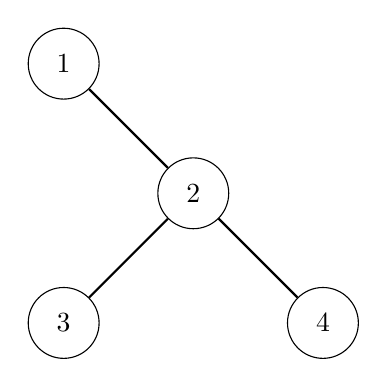
\begin{tikzpicture}
        \node[circle,draw,minimum size=0.9cm,inner sep=0pt](1){$1$};
        \node[circle,draw,minimum size=0.9cm,inner sep=0pt](2)[below right = 1cm and 1cm of 1]{$2$};
        \node[circle,draw,minimum size=0.9cm,inner sep=0pt](3)[below left = 1cm and 1cm of 2]{$3$};
        \node[circle,draw,minimum size=0.9cm,inner sep=0pt](4)[below right = 1cm and 1cm of 2]{$4$};

        \path[draw, thick]
        (1) edge node {} (2)
        (2) edge node {} (3)
        (2) edge node {} (4);
    \end{tikzpicture}
\end{center}
$$V=\{1, 2, 3, 4\},\ E=\{(1, 2), (2, 3), (2, 4)\}$$\\
무방향 그래프(Undirected Graph): 특별한 언급 없으면 무방향 그래프\\
방향 그래프(Directed Graph, Digraph): 선행자? 후속자?\\
단순 그래프(Simple Graph): 루프가 없는 그래프\\
멀티 그래프(Multigraph):
\begin{center}
    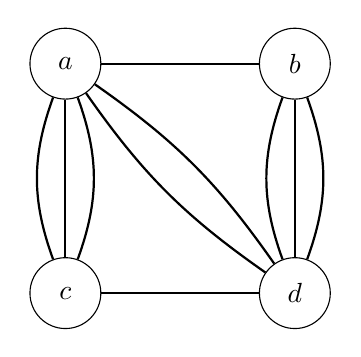
\begin{tikzpicture}
        \node[circle,draw,minimum size=0.9cm,inner sep=0pt](a){$a$};
        \node[circle,draw,minimum size=0.9cm,inner sep=0pt](b)[right = 2cm of a]{$b$};
        \node[circle,draw,minimum size=0.9cm,inner sep=0pt](c)[below = 2cm of a]{$c$};
        \node[circle,draw,minimum size=0.9cm,inner sep=0pt](d)[below = 2cm of b]{$d$};

        \path[draw, thick]
        (a) edge node {} (b)
        (a) edge[bend left = 20] node {} (c)
        (a) edge node {} (c)
        (a) edge[bend right = 20] node {} (c)
        (a) edge[bend left = 10] node {} (d)
        (a) edge[bend right = 10] node {} (d)
        (b) edge node {} (d)
        (b) edge[bend right = 20] node {} (d)
        (b) edge[bend left = 20] node {} (d)
        (c) edge node {} (d)
        ;
    \end{tikzpicture}
\end{center}
연결 그래프(Connected Graph): 모든 Vertex가 연결된 그래프, 모든 Vertex간 경로 존재\\
강한 연결 그래프(Strongly Connected Graph): 방향 그래프에서만, 모든 두 Vertex $v_1, v_2$에 대해 $v_1 \leftrightarrow v_2$\\
연결 요소(Connectivity Component): 그래프에서 모든 Vertex들이 연결되어 있는 부분 그래프

연결 수(Connectivity Number): $G$에서 연결 요소 개수
\newpage
\subsection{그래프 용어}
인접(Adjacent)과 근접(Incident):\\
\begin{center}
    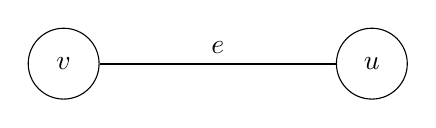
\begin{tikzpicture}
        \node[circle,draw,minimum size=0.9cm,inner sep=0pt](v){$v$};
        \node[circle,draw,minimum size=0.9cm,inner sep=0pt](u)[right = 3cm of v]{$u$};

        \path[draw, thick] (v) edge node[above] {$e$} (u);
    \end{tikzpicture}\\
    $u, v$는 서로 Adjacent, $e$는 $u, v$에 Incident
\end{center}\phantom{}
\\
루프(Loop):\\
\begin{center}
    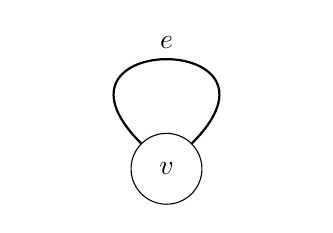
\begin{tikzpicture}
        \tikzset{every loop/.style={}}
        \node[circle,draw,minimum size=0.9cm,inner sep=0pt](v){$v$};
        \path[draw, thick] (v) edge[loop] node[above] {$e$} ();
    \end{tikzpicture}\\
    근접하는 점이 같은 $e$
\end{center}\phantom{}
\\
경로(Path): Vertex들의 열(Sequence) $v_1, v_2, \cdots, v_n$에서 $(v_{k-1}, v_k) \in E, 1 \leq k < n$, 경로의 길이는 $k - 1$

단순 경로(Simple Path): 같은 Edge를 두 번 포함하지 않는 경로

기본 경로(Elementary Path): 같은 Node를 두 번 포함하지 않는 경로
\\\\
사이클(Cycle) 또는 순회(Circuit): $v_1=v_k(k \neq 1)$인 경로, 종점 == 시점

단순 사이클(Simple Cycle): 같은 Edge를 반복해 방문하지 않는 사이클

기본 사이클(Elementary Cycle): 시점 제외 어떤 Node도 반복해 방문하지 않는 사이클
\\\\ 
길이(Length): 경로 또는 사이클을 구성하는 Edge의 수
\\\\
차수(Degree) $d(v)$: Vertex $v$에 근접하는 Edge의 수, Loop는 두 개로 Count

홀수점(Odd Vertex): 차수가 홀수인 Vertex

짝수점(Even Vertex): 차수가 짝수인 Vertex
\\\\
외차수(Out-degree) $out-d(v)$: 방향 그래프에서 Vertex $v$에서 시작하는 화살표 수
\\\\
내차수(In-degree) $in-d(v)$: 방향 그래프에서 Vertex $v$에서 끝나는 화살표 수
\\\\\phantom{}
[정리] 차수에 대한 정리
\begin{itemize}
    \item $G = (V, E)$에서, 모든 Vertex의 차수의 합은 Edge의 수의 두 배이다.
    
    $$\sum_{v \in V} d(v) = 2|E|$$
    \item $G = (V, E)$에서, 차수가 홀수인 정점의 수는 짝수이다.
\end{itemize}

\newpage
\subsection{그래프 vs 트리(Tree)}
\begin{itemize}
    \item 사이클이 없는 그래프
    \item 루트(Root)가 한 개 존재
    \item 루트로부터 다른 모든 Node로 가는 경로가 항상 유일하게 존재
    \item 루트는 모든 트리의 출발점
\end{itemize}

\subsection{오일러 경로(Eulerian Path) 및 오일러 회로(Eulerian Circuit)}
오일러 경로: 멀티 그래프에서 모든 Edge들을 한 번씩만 통과하는 경로를 찾는 문제\\
오일러 회로: Node는 여러 번 통과할 수 있지만, Edge는 한 번씩만 통과하는 사이클\\\\
어떤 그래프 $G$가 오일러 경로를 가지기 위한 필요충분조건은 $G$가 연결 그래프이고, 홀수 차수의 개수가 $0$ 또는 $2$인 경우이다.\\\\
어떤 그래프 $G$가 오일러 회로를 가지기 위한 필요충분조건은 $G$가 연결 그래프이고, 모든 Node들이 짝수 개의 차수를 가지는 경우이다.

\subsection{해밀턴 경로(Hamiltonian Path) 및 해밀턴 회로(Hamiltonian Circuit)}
해밀턴 경로: 그래프에서 모든 Node를 오직 한 번씩만 지나지만 시점으로 돌아오지 않는 경로\\
해밀턴 회로: 그래프에서 모든 Node를 오직 한 번씩만 지나는 순회\\
해밀턴 회로에 대한 충분 조건:
\begin{itemize}
    \item 차수 1을 갖는 Node를 가진 그래프는 해밀턴 순환을 가질 수 없다.
    \item 차수가 2인 Node에 근접하는 두 Vertex는 해밀턴 순환에 포함된다.
    \item 한 Node에 근접하는 두 Vertex가 해밀턴 순환에 포함되면, 그 Node에 근접한 다른 Vertex는 해밀턴 순환에 포함될 수 없다.
\end{itemize}\phantom{}\\
Ore's Theorem: $n \geq 3$일 때, $n$개의 Node를 갖는 단순 연결 그래프 $G$에서 인접하지 않은 임의의 정점 $u, v$에 대해 $d(u) + d(v) \geq n$이면 $G$는 해밀턴 그래프이다.\\\\
Dirac's Theorem: $n \geq 3$일 때, $n$개의 Node를 갖는 단순 연결 그래프 $G$에서 임의의 정점 $v$에 대해 $2d(v) \geq n$이면 $G$는 해밀턴 그래프이다.

\end{document}
